\subsection{۲-الف}
\begin{boxC}
    \begin{equation*}
        \gamma (x) = concat(Unary(\left Binary(x) \right - 1), Binary(x))
    \end{equation*}

    \begin{equation*}
        \delta (x) = concat(\gamma (\left Binary(x) \right - 1), Binary(x))
    \end{equation*}

    
    \begin{equation*}
        9 = (1001)_{Binary}    
    \end{equation*}

    \begin{equation*}
        9 = (1110 , 001)_{\gamma}    
    \end{equation*}

    \begin{equation*}
        9 = (10 , 1 , 001)_{\delta}    
    \end{equation*}


    \begin{equation*}
        100 = (1100100)_{Binary}    
    \end{equation*}

    \begin{equation*}
        100 = (1111110 , 100100)_{\gamma}    
    \end{equation*}

    \begin{equation*}
        9 = (110 , 10 , 100100)_{\delta}    
    \end{equation*}
    
\end{boxC}

\newpage

\subsection{۲-ب}
\begin{boxC}
    \begin{equation*}
        \left | \gamma (x) \right | = \left | \delta (x) \right |        
    \end{equation*}

    \begin{equation*}
        \left | Unary(Binary(x) - 1) \right | 
        +
        \left | Binary(x) \right |
        =
        \left | \gamma (x) \right |
        +
        \left | Binary(x) \right |   
    \end{equation*}

    \begin{equation*}
        \left | Unary(Binary(x) - 1) \right | 
        =
        \left | \gamma (x) \right |
    \end{equation*}


    \begin{equation*}
        2 \log (\log (x)) + 1 = \log (x) + 1 
    \end{equation*}

    \begin{equation*}
        \log (x) = x - 4
    \end{equation*}

    \begin{equation*}
        x = 4.699
    \end{equation*}
    
\end{boxC}


\subsection{۲-ج}

\begin{figure}[h]
    \centering
    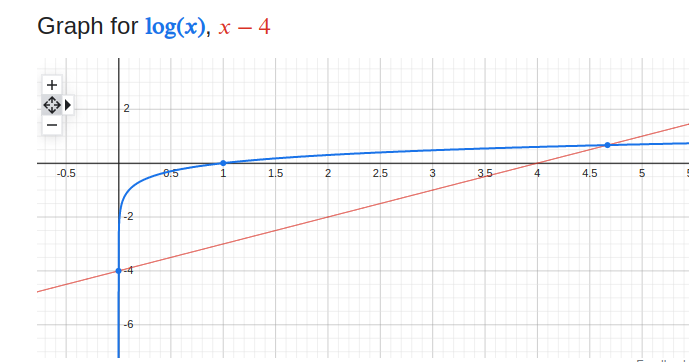
\includegraphics
    [width = 0.8\textwidth]
    {IR3/images/2-2-plot.png}
    \caption{رسم نمودار طول کدهای گاما و دلتا}
    \label{fig:enter-label}
\end{figure}

\begin{boxC}
    با توجه به نمودار بالا کاملا به صورت شهودی قضیه مدنظر سوال اثبات می‌شود که از نقطه حدودا ۴.۶ به بعد 
    طول کد رشته دلتای هر عدد از طول رشته گاما کوچکتر است.
\end{boxC}